\documentclass[a4paper, 12pt,
bibliography=totoc,           % Lit.verz. ins Inh.verz.
numbers=noenddot,   % Kein Punkt nach letzter Gliederungsziffer
]{scrartcl}

% Für Texte in deutscher Sprache
\usepackage[utf8]{inputenc}
\usepackage{csquotes}
\usepackage[T1]{fontenc}
\usepackage[a4paper, left=2cm, right=3cm, top=3cm, bottom=3cm]{geometry}

\usepackage{physics}
\usepackage{amsthm}

\theoremstyle{definition}
\newtheorem{definition}{Definition}[section]
\newtheorem{eg}{Example}[section]
\newtheorem{note}{Note}[section]
\newtheorem{theorem}{Theorem}[section]
\newtheorem{corollary}{Corollary}[section]
\newtheorem{proposition}{Proposition}[section]

\theoremstyle{remark}
\newtheorem*{statement}{Statement}

\usepackage{listings}
\usepackage{color}

\usepackage[backend=biber, style=verbose]{biblatex}
\usepackage{hyperref}
\addbibresource{kapitel/05_literatur.bib} % Replace with the path to your .bib file
% Custom command to change punctuation between fields
\renewcommand*{\newunitpunct}{\addcomma\space}

% Custom bibliography driver for @misc entries
\DeclareBibliographyDriver{misc}{%
  \printnames{author}%
  \setunit{\labelnamepunct}\newblock
  \printfield{title}%
  \newunit\newblock
  \printfield{howpublished}%
  \newunit\newblock
  \printfield{note}%
  \finentry
}

\definecolor{dkgreen}{rgb}{0,0.6,0}
\definecolor{gray}{rgb}{0.5,0.5,0.5}
\definecolor{mauve}{rgb}{0.58,0,0.82}

% Grafiken und Bilder einbinden
\usepackage{graphicx}

% Pakete für Mathe-Umgebungen, -Symbole und -Schriftstile
\usepackage{amsfonts}
\usepackage{amssymb}
\usepackage{amsmath}
\usepackage{gensymb}
\usepackage{extpfeil}
\usepackage{amsthm}

\usepackage{xurl}
\usepackage{xcolor,cancel}
\usepackage{xfrac}
\usepackage{tikz}
\usepackage{mathrsfs}
\usepackage{tabularx}
\usepackage{extarrows}
\usepackage{array}
\usepackage{enumitem}

\newcommand\hcancel[2][black]{\setbox0=\hbox{$#2$}%
\rlap{\raisebox{.45\ht0}{\textcolor{#1}{\rule{\wd0}{1pt}}}}#2} 

\usepackage{svg}
\usepackage{float}

% Absatzeinzug und -abstand
\parindent 0pt	% Einzug
\parskip 6pt	% Abstand

% Links und Verweise innerhalb von PDF Dokumenten
\usepackage{hyperref}

% Trennungsregeln
\hyphenation{Sil-ben-trenn-ung}

% Helvetica als Standard-Dokumentschrift
%\usepackage[scaled]{helvet}
%\renewcommand{\familydefault}{\sfdefault}

% Latin Modern Sans als Standard-Dokumentschrift
\usepackage{lmodern}
\renewcommand{\familydefault}{\sfdefault}

\usepackage{graphicx}
\usepackage{subcaption} % Paket für subfigures
\usepackage{float}

\usepackage{adjustbox} % für die vertikale Zentrierung

\usepackage{pdfpages}

\definecolor{codegreen}{rgb}{0,0.6,0}
\definecolor{codegray}{rgb}{0.5,0.5,0.5}
\definecolor{codepurple}{rgb}{0.58,0,0.82}
\definecolor{backcolour}{rgb}{0.95,0.95,0.92}

% Define C# style
\lstdefinestyle{csharp}{
    language=[Sharp]C,
    basicstyle=\ttfamily\footnotesize,
    keywordstyle=\color{blue},
    commentstyle=\color{gray},
    stringstyle=\color{red},
    numbers=left,
    numberstyle=\tiny\color{gray},
    stepnumber=1,
    numbersep=5pt,
    tabsize=4,
    showspaces=false,
    showstringspaces=false,
    frame=single,
    breaklines=true
}

% Set the default style for all listings to C# style
\lstset{style=csharp}


% Hier Namen etc. einsetzen
\newcommand{\studentzwei}{Patrick Mayer}
\newcommand{\emailzwei}{m.patrick.international@gmail.com}
\newcommand{\versuchsname}{Couple Theory}

% Define a custom command for non-italics
\newcommand{\nonitalic}[1]{\,\mathrm{#1}}

% Define specific units
\newcommand{\kg}{\nonitalic{kg}}
\newcommand{\m}{\nonitalic{m}}
\newcommand{\s}{\nonitalic{s}}
\newcommand{\cm}{\nonitalic{cm}}
\newcommand{\mm}{\nonitalic{mm}}
\newcommand{\Pa}{\nonitalic{Pa}}
\newcommand{\GPa}{\nonitalic{GPa}}
\newcommand{\N}{\nonitalic{N}}
\newcommand{\J}{\nonitalic{J}}
\newcommand{\V}{\nonitalic{V}}
\newcommand{\A}{\nonitalic{A}}
\newcommand{\C}{\nonitalic{C}}
\newcommand{\F}{\nonitalic{F}}
\newcommand{\g}{\nonitalic{g}}
\newcommand{\liter}{\nonitalic{l}}
\newcommand{\e}{\nonitalic{e}}
\newcommand{\mol}{\nonitalic{mol}}
\newcommand{\K}{\nonitalic{K}}
\newcommand{\cd}{\nonitalic{cd}}
\newcommand{\mN}{\nonitalic{mN}}
\newcommand{\cel}{\nonitalic{C}}
%for normal differentials
\newcommand{\diff}{\nonitalic{d}}
%for E (+-) numbers
\newcommand{\E}{\nonitalic{E}}

\DeclareMathOperator{\Eig}{Eig}
\DeclareMathOperator{\Kern}{Kern}

% Increase ToC depth and section numbering depth
\setcounter{tocdepth}{5}
\setcounter{secnumdepth}{5}

% Define new sectioning commands
\newcommand{\subsubsubsection}[1]{\paragraph{#1}\mbox{}\\}
\newcommand{\subsubsubsubsection}[1]{\subparagraph{#1}\mbox{}\\}

\begin{document}

% Titelseite
\begin{titlepage}

\begin{center}
    \begin{minipage}[c]{0.4\textwidth}
        \adjustbox{valign=c}{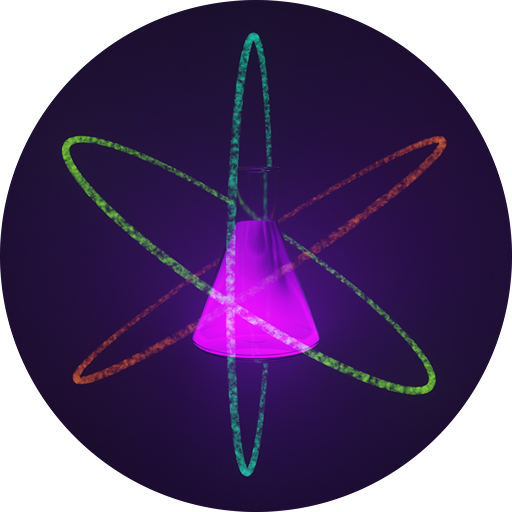
\includegraphics[scale=0.15]{bilder/logo.png}}
    \end{minipage}%
    \hfill
    \begin{minipage}[c]{0.25\textwidth}
        \adjustbox{valign=c}{\textbf{\Huge Poimora}}
    \end{minipage}
\end{center}

\begin{center}
\vspace{3.0cm}
Theory \\[0.6cm]
{\LARGE \textbf{\versuchsname}}

\vspace{3.0cm}
Elaborated and written by \\[0.2cm]
\textbf{\studentzwei} \\ 
(\emailzwei)

\vspace{5.0cm}
On Behalf of\\[0.2cm]
\textbf{Poimora} resp. \textbf{Poimora Science} \\
(poimora.science@gmail.com)

\end{center}
\end{titlepage}



% Inhaltsverzeichnis
\tableofcontents


% Hier Kapitel einbinden
\newpage
\section{Introduction}
\label{sec:en:introduction}

This theory sheet models the transition from single to couple. And maybe more couple-shaded theorems.

Those theorems may be questionable on their own but they guarantee everbody a partner candidate while not guaranteeing a partner.

This sheet is a theoretical model to train creating models with a goal and proving it on the way if a proof seems sensible.
\newpage
\section{Couple Theory}
\label{sec:en:theory}

\subsection{Single To Couple Transition}

\begin{definition}[Human Sets]\label{sec:en:definition:human-sets}
    \leavevmode\\
    Let $\mathbb{H}$ be the set of humans, and $\mathbb{S}\subseteq\mathbb{H}$ the set of human singles.
   
    Let $\equiv:\;\mathbb{H}^2\times\mathbb{H}^2\rightarrow\{0,1\},\;((x,y),(u,v))\mapsto (x=u\,\land\,y=v)\,\lor\,(x=v\,\land\,y=u)$ such that
    $(x,y)\equiv(u,v)\Longleftrightarrow(x=u\,\land\,y=v)\,\lor\,(x=v\,\land\,y=u)$.
    
    Let $\mathcal{H}^2:=\left\{ (x,y)\in\mathbb{H}^2 \;\middle|\; x\neq y \,\land\, (x,y)\equiv(y,x) \right\}$.
    
    Let $\mathcal{S}^2:=\left\{ (x,y)\in\mathbb{S}^2 \;\middle|\; x\neq y \,\land\, (x,y)\equiv(y,x) \right\}$.
    
    This means different people, can be arranged in whatever oder you like and are never the same.
    
    Therefore for $\mathcal{H}^2$ and $\mathcal{S}^2$ follows that:
    \begin{align*}
        (x,y)\equiv(y,x) &\nRightarrow x = y \\
        (x,y)\equiv(y,x) &\nRightarrow(x,y)=(y,x).
    \end{align*}

    Furthermore one has $(x,y)\equiv(y,x)\land x\neq y\land (x,y)\neq(y,x)$.
\end{definition}

\begin{theorem}[Couple Identity Is an Equivalence Relation]
    \leavevmode\\
    Let $\mathbb{H}$ be a set and define $\forall(x,y),(u,v)\in\mathbb{H}^2$:
    $$(x,y)\equiv(u,v) \Longleftarrow (x=u\,\land\,y=v)\,\lor\,(x=v\,\land\,y=u).$$
    Then $\equiv$ is an equivalence relation on $\mathbb{H}^2$.
    \begin{proof}
        \leavevmode\\
        \begin{enumerate}
            \item \parbox[t]{\linewidth}{
                Reflexivity

                \medskip

                Let $(x,y)\in\mathbb{H}^2$.

                \medskip

                Since $x=x$ and $y=y$, it follows that
                $(x,y)\equiv(x,y)$.

                \medskip
                
                Thus, $\equiv$ is reflexive.
            }
            \item \parbox[t]{\linewidth}{
                Symmetry

                \medskip

                Let $(x,y),(u,v)\in\mathbb{H}^2$ and consider

                \medskip

                $$(x,y)\equiv(u,v)$$.

                \medskip

                By definition either $x=u\land y=v$ or $x=v\land y=u$.

                \medskip

                By the definition of equality both cases can be $u=x\land v=y$ or $u=y\land v=x$.

                Hence $(u,v)\equiv(x,y)$.

                \medskip

                Thus, $\equiv$ is symmetric.
            }
            \item \parbox[t]{\linewidth}{
                Transitivity

                \medskip

                Let $(x,y),(u,v),(a,b)\in\mathbb{H}^2$ and consider

                \medskip

                $$(x,y)\equiv(u,v) \quad \land \quad (u,v)\equiv(a,b).$$

                \medskip

                There are four possible combinations per equivalence:

                \medskip

                \begin{center}
                    \begin{tabular}{c|c|c}
                        \textbf{First Equivalence} &
                        \textbf{Second Equivalence} &
                        \textbf{Consequence} \\
                        \hline
                        $x=u$, $y=v$ &
                        $u=a$, $v=b$ &
                        $x=a$, $y=b$ \\

                        $x=u$, $y=v$ &
                        $u=b$, $v=a$ &
                        $x=b$, $y=a$ \\

                        $x=v$, $y=u$ &
                        $u=a$, $v=b$ &
                        $x=b$, $y=a$ \\

                        $x=v$, $y=u$ &
                        $u=b$, $v=a$ &
                        $x=a$, $y=b$
                    \end{tabular}
                \end{center}

                \medskip

                In every case $(x=a\,\land\,y=b)\,\lor\,(x=b\,\land\,y=a)$

                Hence $(x,y)\equiv(a,b)$.

                \medskip

                Thus, $\equiv$ is transitive.
            }
        \end{enumerate}
        Since $\equiv$ is reflexive, symmetric, and transitive, it is an equivalence relation on $\mathbb{H}^2$.
    \end{proof}
\end{theorem}

\begin{theorem}[Order Theorem]\label{sec:en:theorem:order-theorem}
    \leavevmode\\
    A couple preserves its identity without making the ordered tuples equal.
    \begin{statement}
        For every $(x,y)\in\mathcal{H}^2$:
        $$(x,y)\equiv(y,x)\,\land\,(x,y)\neq(y,x).$$
    \end{statement}
    \begin{proof}
        Let $(x,y)\in\mathcal{H}^2$. By definition $x\neq y$. Moreover:
        $$(x,y)\equiv(y,x)$$
        because the second disjunct in the definition of $\equiv$ is satisfied.
        
        Suppose, for contradiction, that
        $$(x,y)=(y,x).$$
        By equality of ordered pairs, $x=y$, contradicting $x\neq y$.
        
        Hence:
        $$(x,y)\neq(y,x).$$

        Therefore $(x,y)\equiv(y,x)\,\land\,(x,y)\neq(y,x)$.
    \end{proof}
\end{theorem}

\begin{corollary}
    A tuple can be identical without being equals, as an identical couple isn't contingent to the individual's order in a list. Identical couple with identical humans but different positions in the list.
\end{corollary}

\begin{theorem}[Single Set Inclusion]\label{sec:en:theorem:single-set-inclusion}
    Since $\mathcal{S}^2$ and $\mathcal{H}^2$ emerge from $\mathbb{S}\subseteq\mathbb{H}$, the same inclusion applies for the emergent sets.
    \begin{statement}
        Since $\mathbb{S}\subseteq\mathbb{H}$, we have $\mathcal{S}^2\subseteq\mathcal{H}^2$.
    \end{statement}
    \begin{proof}
        Let $(x,y)\in\mathcal{S}^2$.
        
        Then $x,y\in\mathbb{S}$, $x\neq y$, and $(x,y)\equiv(y,x)$.
        
        Since $\mathbb{S}\subseteq\mathbb{H}$, we have $x,y\in\mathbb{H}$. Thus $(x,y)\in\mathbb{H}^2$
        
        Since the conditions applied by $\mathcal{S}^2$, we have $x\neq y$, and $(x,y)\equiv(y,x)$, which is sufficient for $(x,y)\in\mathcal{H}^2$.

        Therefore $\mathcal{S}^2\subseteq\mathcal{H}^2$.
    \end{proof}
\end{theorem}

\begin{definition}[Extended Human Sets]\label{sec:en:definition:extended-human-sets}
    \leavevmode\\
    Let $\perp\notin\mathbb{H}$ be an nonexistent or unavailable human, and $\triangle\notin\mathbb{H}^2\,\land\,\triangle\notin\mathcal{H}^2$ with $\triangle:=(\perp,\perp)$ an nonexistent couple.
    Let $\hat{\mathbb{H}}^2:=\mathbb{H}^2\cup\{\triangle\}$, $\hat{\mathcal{H}}^2:=\mathcal{H}^2\cup\{\triangle\}$, and $\hat{\mathbb{S}}:=\mathbb{S}\cup\{\perp\}$ with continuing validity of the equivalence.

    Therefore let
    $$\equiv:\;\hat{\mathbb{H}}^2\times\hat{\mathbb{H}}^2\rightarrow\{0,1\},\;((x,y),(u,v))\mapsto (x=u\,\land\,y=v)\,\lor\,(x=v\,\land\,y=u)$$
    such that
    $$(x,y)\equiv(u,v)\Longleftrightarrow(x=u\,\land\,y=v)\,\lor\,(x=v\,\land\,y=u).$$
\end{definition}

\begin{theorem}[Preservation of the Couple Equivalence]
    \begin{statement}
        The relation $\equiv$ defined on $\hat{\mathbb{H}}^2$ is an equivalence relation and extends the original relation on $\mathbb{H}^2$.
    \end{statement}
    \begin{proof}
        Every element of $\hat{\mathbb{H}}^2$ is an ordered pair, since $\triangle=(\perp,\perp)$. Therefore the definition
        $$(x,y)\equiv(u,v)\Longleftrightarrow(x=u\,\land\,y=v)\,\lor\,(x=v\,\land\,y=u)$$
        applies to every pair of elements of the extended set.

        Reflexivity, symmetry, and transitivity follow by exactly the same argument as for Definition \ref{sec:en:definition:human-sets}, using the reflexivity, symmetry, and transitivity of equality.

        Furthermore, for all \(a,b\in\mathbb H^2\), the defining condition for \(a\equiv b\) is unchanged. Hence the extended relation agrees with the original relation on \(\mathbb H^2\).
    \end{proof}
\end{theorem}

\begin{proposition}[Isolation of the Nonexistent Couple]
    \begin{statement}
        $$\forall c\in\hat{\mathbb{H}}^2:\;c\equiv\triangle\Longleftrightarrow c=\triangle$$.
    \end{statement}
    \begin{proof}
        Let $c=(x,y)\in\hat{\mathbb{H}}^2$. By definition \ref{sec:en:definition:extended-human-sets}:
        $$\triangle=(\perp,\perp).$$
        Thus:
        \begin{align*}
            c\equiv\triangle &\Longleftrightarrow (x,y) \equiv (\perp,\perp) \\
            &\Longleftrightarrow (x=\perp\,\land\,y=\perp) \\
            &\Longleftrightarrow (x,y) = (\perp,\perp) \\
            &\Longleftrightarrow c = \triangle.
        \end{align*}
        Therefore $[\triangle]_\equiv=\{\triangle\}$.
    \end{proof}
\end{proposition}

\begin{corollary}
    No real human couple is equivalent to the nonexistent couple.
\end{corollary}

\begin{proposition}[The Extension Preserves the Original Human Couples]
    \begin{statement}
        $$\hat{\mathcal{H}}^2\setminus\{\triangle\}=\mathcal{H}^2.$$
    \end{statement}
    \begin{proof}
        By definition \ref{sec:en:definition:extended-human-sets}:
        $$\hat{\mathcal{H}}^2=\mathcal{H}^2\cup\{\triangle\}.$$
        Since $\triangle\notin\mathcal{H}^2$:
        \begin{align*}
            \hat{\mathcal{H}}^2\setminus\{\triangle\} &= (\mathcal{H}^2\cup\{\triangle\})\setminus\{\triangle\} \\
            &= \mathcal{H}^2.
        \end{align*}
    \end{proof}
\end{proposition}

\begin{proposition}[The Extension Preserves the Original Human Singles]
    \begin{statement}
        $$\hat{\mathbb{S}}\setminus\{\perp\}=\mathbb{S}.$$
    \end{statement}
    \begin{proof}
        By definition \ref{sec:en:definition:extended-human-sets}:
        $$\hat{\mathbb{S}}=\mathbb{S}\cup\{\perp\}.$$
        Since $\perp\notin\mathbb{S}$:
        \begin{align*}
            \hat{\mathcal{S}}\setminus\{\perp\} &= (\mathbb{S}\cup\{\perp\})\setminus\{\perp\} \\
            &= \mathbb{S}.
        \end{align*}
    \end{proof}
\end{proposition}

\begin{definition}[Single-Couple Transformation]\label{sec:en:definition:single-couple-transformation}
    \leavevmode\\
    Let $\mathcal{C}:\;\mathcal{S}^2\rightarrow\mathcal{H}^2$.

    $\mathcal{C}$ transforms $\mathbb{S}$ to $\mathbb{S}'$ such that 
    $$\mathcal{C}:\;\mathcal{S}^2\rightarrow\mathcal{H}^2,\;(s_1,s_2)\mapsto(s_1,s_2),$$ 
    and $\mathbb{S}'=\mathbb{S}\setminus\{s_1,s_2\}$

    with $s_1,s_2\in\mathbb{S}\,\land\,s_1,s_2\notin\mathbb{S}'$ where $\mathbb{S}'\subseteq\mathbb{H}$ is the transformed set $\mathbb{S}$.
\end{definition}

\begin{proposition}[Well-Definedness of the Single-Couple Transformation]\label{sec:en:prop:well-def-sct}
    \begin{statement}
        The mapping
        $$\mathcal{C}:\,\mathcal{S}^2\rightarrow\mathcal{H}^2$$
        is well-defined.
    \end{statement}
    \begin{proof}
        Let $(s_1,s_2)\in\mathcal{S}^2$.
        
        By theorem \ref{sec:en:theorem:single-set-inclusion} $\mathcal{S}^2\subseteq\mathcal{H}^2$.

        By definition \ref{sec:en:definition:single-couple-transformation}
        $$\mathcal{C}(s_1,s_2)=(s_1,s_2).$$
        
        Thus $\mathcal{C}(s_1,s_2)\in\mathcal{H}^2.$
        
        Furthermore, the mapping assigns exactly one output to every element of \(\mathcal S^2\).
        
        Hence \(\mathcal C\) is a well-defined function.
    \end{proof}
\end{proposition}

\begin{proposition}[Correctness of the Single-Couple Transition]
    \begin{statement}
        For every $(s_1,s_2)\in\mathcal{S}^2$, the transformation satisfies
        $$s_1,s_2\notin\mathbb{S}'\,\land\,\mathbb{S}'\subseteq\mathbb{S}.$$
    \end{statement}
    \begin{proof}
        By definition \ref{sec:en:definition:single-couple-transformation}
        $$\mathbb{S}'=\mathbb{S}\setminus\{s_1,s_2\}.$$
        By definition of set difference
        $$\forall z\in\mathbb S': z\in\mathbb S\land z\notin\{s_1,s_2\}.$$

        Thus
        $$s_1,s_2\notin\mathbb S'.$$

        By the definition of a subset, we have
        $$\mathbb{S}'\subsetneq\mathbb{S} \Longleftrightarrow \forall z(z\in\mathbb{S}'\Rightarrow\in\mathbb{S}),$$

        By Definition \ref{sec:en:definition:single-couple-transformation},
        $$z\in\mathbb S'\iff z\in\mathbb S\setminus\{s_1,s_2\}.$$

        By the definition of set difference,
        $$
        z\in\mathbb S\setminus\{s_1,s_2\}
        \iff
        z\in\mathbb S\land z\notin\{s_1,s_2\}.
        $$

        In particular
        $$z\in\mathbb S.$$

        Since $z$ was arbitrary
        $$\forall z\,(z\in\mathbb S'\implies z\in\mathbb S).$$
        Therefore
        $$\mathbb S'\subseteq\mathbb S.$$
        Therefore $s_1,s_2\notin\mathbb S'\land\mathbb S'\subseteq\mathbb S$.
    \end{proof}
\end{proposition}

\begin{proposition}[Order Independence of the Single-Couple Transformation]
    \begin{statement}
        For every $(s_1,s_2)\in\mathcal S^2$:
        $$\mathcal C(s_1,s_2)\equiv\mathcal C(s_2,s_1).$$.

        Moreover, both transformations yield the same singles set.
    \end{statement}
    \begin{proof}
        By Definition \ref{sec:en:definition:single-couple-transformation}
        \begin{align*}
            \mathcal C(s_1,s_2)&=(s_1,s_2),\\
            \mathcal C(s_2,s_1)&=(s_2,s_1).
        \end{align*}

        By Theorem \ref{sec:en:theorem:order-theorem}
        $$(s_1,s_2)\equiv(s_2,s_1).$$

        Therefore
        $$\mathcal C(s_1,s_2)\equiv\mathcal C(s_2,s_1).$$

        For the state transitions, we have
        \begin{align*}
            \mathbb S'_1&=\mathbb S\setminus\{s_1,s_2\},\\
            \mathbb S'_2&=\mathbb S\setminus\{s_2,s_1\}.
        \end{align*}

        Since unordered sets satisfy
        $$\{s_1,s_2\}=\{s_2,s_1\},$$

        it follows that
        $$\mathbb S'_1=\mathbb S'_2.$$
    \end{proof}
\end{proposition}

\begin{proposition}[Injectivity of the Couple Creator]
    \begin{statement}
        The function $\mathcal C$ is injective.
    \end{statement}
   
    \begin{proof}
        Let $(s_1,s_2),(t_1,t_2)\in\mathcal S^2$ and suppose
        $$\mathcal C(s_1,s_2)=\mathcal C(t_1,t_2).$$

        By Definition \ref{sec:en:definition:single-couple-transformation}
        $$(s_1,s_2)=(t_1,t_2).$$

        By equality of ordered pairs $s_1=t_1\land s_2=t_2.$

        Hence
        $$\mathcal C(s_1,s_2)=\mathcal C(t_1,t_2)
        \implies
        (s_1,s_2)=(t_1,t_2).$$

        Therefore $\mathcal C\text{ is injective}.$
    \end{proof}
\end{proposition}

\begin{corollary}
    Injectivity uses actual equality $=$, not the couple equivalence $\equiv$.

    Indeed $\mathcal C(s_1,s_2)\equiv\mathcal C(s_2,s_1)$ does not violate injectivity, because for $s_1\ne s_2$,
    $$\mathcal C(s_1,s_2)\ne\mathcal C(s_2,s_1).$$
\end{corollary}

\begin{proposition}[Surjectivity of the Couple Creator]
    \begin{statement}
        The function $\mathcal C$ is surjective if and only if
        $$\mathcal S^2=\mathcal H^2.$$
    \end{statement}
   
    \begin{proof}
        By Definition \ref{sec:en:definition:single-couple-transformation}, the image of $\mathcal C$ is
        $$\operatorname{im}(\mathcal C)
        =
        \{\mathcal C(s_1,s_2):(s_1,s_2)\in\mathcal S^2\}.$$

        Since $\mathcal C(s_1,s_2)=(s_1,s_2)$, we have $\operatorname{im}(\mathcal C)=\mathcal S^2.$

        By definition, $\mathcal C$ is surjective onto $\mathcal H^2$ precisely when $\operatorname{im}(\mathcal C)=\mathcal H^2.$

        Therefore 
        $$\mathcal C\text{ is surjective}\iff\mathcal S^2=\mathcal H^2.$$
    \end{proof}
\end{proposition}

\begin{proposition}[Bijectivity of the Couple Creator]
    \begin{statement}
        $$\mathcal C\text{ is bijective}
            \iff
            \mathcal S^2=\mathcal H^2.$$
    \end{statement}
    \begin{proof}
        A function is bijective if and only if it is both injective and surjective.

        We have already established that $\mathcal C$ is always injective.

        Furthermore
        $$\mathcal C\text{ is surjective}
            \iff
            \mathcal S^2=\mathcal H^2.$$

        Therefore
        $$\mathcal C\text{ is bijective}
            \iff
            \mathcal S^2=\mathcal H^2.$$
    \end{proof}
\end{proposition}

\begin{definition}[Date-Couple-Relation]\label{sec:en:definition:date-couple-relation}
    Since theorem \ref{sec:en:theorem:date-couple-relation}, it follows that $\exists\mathcal{D}$ such that
    $$\mathcal{D}:\;\mathbb{S}\times\hat{\mathbb{S}}\rightarrow\hat{\mathcal{H}}^2,\;(x,y)\mapsto\begin{cases}\mathcal{C}(x,y),\quad &\text{if }x\neq y\,\land\,y\neq\perp \\ \triangle,\quad &\text{else.}\end{cases}$$
    with the state-transition 
    $$\mathbb{S}'=\begin{cases} \mathbb{S}\setminus\{x,y\},\quad &\mathcal{D}(x,y)\in\mathcal{H}^2 \\ \mathbb{S},\quad &\mathcal{D}(x,y)=\triangle. \end{cases}$$
\end{definition}

\begin{proposition}
    \begin{statement}
        The function $\mathcal D$ is well-defined.
    \end{statement}
    \begin{proof}
        Let $(x,y)\in\mathbb S\times\hat{\mathbb S}$ be arbitrary.

        Case 1: Suppose $x\neq y\land y\neq\perp$.

        Since $x\in\mathbb S$ and $y\in\hat{\mathbb S}=\mathbb S\cup\{\perp\}$, the condition $y\neq\perp$ implies $y\in\mathbb S$.

        Together with $x\neq y$, this yields
        $$(x,y)\in\mathcal S^{2}.$$

        Therefore, $\mathcal C(x,y)$ is defined. By Definition 2.3 and Theorem 2.3,
        $$\mathcal D(x,y)=\mathcal C(x,y)
            =(x,y)\in\mathcal H^{2}
            \subseteq\hat{\mathcal H}^{2}.
            $$

        Case 2: Suppose $x=y\lor y=\perp$.

        By Definition \ref{sec:en:definition:date-couple-relation} $\mathcal D(x,y)=\triangle.$

        By Definition \ref{sec:en:definition:extended-human-sets} $\triangle\in\hat{\mathcal H}^{2}.$

        Thus, in both cases $\mathcal D(x,y)\in\hat{\mathcal H}^{2}.$

        Since the cases are mutually exclusive and exhaustive, every input has exactly one output. Hence $\mathcal D$ is well-defined.
    \end{proof}
\end{proposition}

\begin{theorem}[Existence of a Date-Couple-Relation]\label{sec:en:theorem:date-couple-relation}
    $$\forall x\in\mathbb{S}\subseteq\mathbb{H}:\;\exists y\in\hat{\mathbb{S}}\setminus\{x\}:\;(x,y)\mapsto(x,y)\in\mathcal{H}^2$$
    via the $\mathcal{C}$ transformation, unless $y=\perp$, then $(x,y)\mapsto \triangle\,\land\,\mathbb{S}'=\mathbb{S}$.

    \begin{statement}
        Therefore there must exist at least one $\mathcal{D}$ extending $\mathcal{C}$.
        Therefore
        $$\exists\mathcal D:
            \mathbb S\times\hat{\mathbb S}
            \longrightarrow\hat{\mathcal H}^2
            \quad\text{such that}\quad
            \mathcal D|_{\mathcal S^2}=\mathcal C.$$
        must hold.
    \end{statement}
    \begin{proof}
        Let $x\in\mathbb S$ be arbitrary.

        By Definition \ref{sec:en:definition:extended-human-sets},
        $$\hat{\mathbb S}=\mathbb S\cup\{\perp\},
            \qquad \perp\notin\mathbb H.$$

        Since $\mathbb S\subseteq\mathbb H$, it follows that
        $$\perp\notin\mathbb S.$$

        In particular, we have
        $$\perp\neq x.$$

        Moreover, $\perp\in\hat{\mathbb S}$. Therefore
        $$\perp\in\hat{\mathbb S}\setminus\{x\}.$$

        Hence there exists at least one $y\in\hat{\mathbb S}\setminus\{x\}$, namely $y=\perp$.

        We distinguish two cases.
        Case 1: $y\neq\perp$
        Since $y\in\hat{\mathbb S}=\mathbb S\cup\{\perp\}$ and $y\neq\perp$, we obtain
        $$y\in\mathbb S.$$

        Furthermore, $y\neq x$. Thus, we have
        $$ (x,y)\in\mathcal S^2.$$

        By Definition \ref{sec:en:definition:single-couple-transformation}, the Couple Creator is applicable:
        $$\mathcal C(x,y)=(x,y).$$

        By Proposition \ref{sec:en:prop:well-def-sct}, $\mathcal C$ is well-defined, so $\mathcal C(x,y)\in\mathcal H^2.$

        The accompanying state transition is $\mathbb S'=\mathbb S\setminus\{x,y\}.$

        Case 2: \(y=\perp\)
        By Definition \ref{sec:en:definition:extended-human-sets}
        $$\triangle=(\perp,\perp).$$

        Since $\perp\notin\mathbb H$
        $$(x,\perp)\notin\mathcal S^2. $$

        Consequently, the Couple Creator $\mathcal C$ cannot be applied to $(x,\perp)$.

        Instead, the model assigns the nonexistent couple $(x,\perp)\longmapsto\triangle$ and leaves the singles set unchanged:
        $$\mathbb S'=\mathbb S.$$

        Thus, for every $x\in\mathbb S$, at least one candidate $y\in\hat{\mathbb S}\setminus\{x\}$ exists, and the model specifies either a valid couple formation or the nonexistent-couple outcome.

        Therefore, the stated candidate-existence property holds.

        Let $(s_1,s_2)\in\mathcal S^{2}$. By Definition \ref{sec:en:definition:human-sets},
        $s_1\neq s_2$

        and, since $s_2\in\mathbb S\subseteq\mathbb H$ while $\perp\notin\mathbb H$,
        $s_2\neq\perp.$

        Therefore, the first case of Definition \ref{sec:en:definition:date-couple-relation} applies:
        $$\mathcal D(s_1,s_2)=\mathcal C(s_1,s_2).$$

        Since $(s_1,s_2)$ was arbitrary, $\mathcal D|_{\mathcal S^{2}}=\mathcal C.$

        Thus the function specified in Definition \ref{sec:en:definition:date-couple-relation} exists and extends $\mathcal C$. Therefore:
        $$\exists\mathcal D:
            \mathbb S\times\hat{\mathbb S}
            \longrightarrow\hat{\mathcal H}^{2}
            \quad\text{such that}\quad
            \mathcal D|_{\mathcal S^{2}}=\mathcal C.$$
    \end{proof}
\end{theorem}

\begin{corollary}
    Whenever $\mathcal D(x,y)=\mathcal C(x,y)$, both remove $\{x,y\}$ from $\mathbb S$. In the failure case, Definition \ref{sec:en:definition:date-couple-relation} leaves $\mathbb S$ unchanged.
\end{corollary}

\begin{corollary}[Guaranteed Partner Candidate; Not Guaranteed Partner Principle]\label{sec:en:corollary:guaranteed-partner-candidate-not-guaranteed-partner-principle}
    \leavevmode\\
    You're guaranteed to find a partner as long as you allow that partner to be unavailable or nonexistent. But if your partner is unavailable or nonexistent, though, you aren't considered taken or a human in a couple.
    \begin{align*}
        \mathcal{D}(x,y)\in\mathcal{H}^2&\Longrightarrow x,y\notin\mathbb{S}'.\\
        \mathcal{D}(x,y)=\triangle&\Longrightarrow x\in\mathbb{S}'\,\land\,\mathbb{S}'=\mathbb{S}.
    \end{align*}
    \begin{proof}
        Let $(x,y)\in\mathbb S\times\hat{\mathbb S}$ be arbitrary.

        1. Successful date

        Suppose $\mathcal D(x,y)\in\mathcal H^2.$

        By Definition \ref{sec:en:definition:date-couple-relation}, this implies that the successful case applies, and therefore
        $$\mathbb S'=\mathbb S\setminus\{x,y\}.$$

        By the definition of set difference
        $$\forall z:\quad
            z\in\mathbb S'
            \iff
            z\in\mathbb S\land z\notin\{x,y\}.$$

        In particular, since
        $$x\in\{x,y\}
            \quad\land\quad
            y\in\{x,y\},$$

        we obtain
        $$x\notin\mathbb S'
            \quad\land\quad
            y\notin\mathbb S'.$$

        Hence $\mathcal D(x,y)\in\mathcal H^2\implies x,y\notin\mathbb S'.$

        2. Unsuccessful date

        Suppose $\mathcal D(x,y)=\triangle.$

        By Definition 2.4, the state-transition rule gives $\mathbb S'=\mathbb S.$

        Since $(x,y)\in\mathbb S\times\hat{\mathbb S}$, we know that $x\in\mathbb S.$

        Consequently, because $\mathbb S'=\mathbb S$, we have $x\in\mathbb S'.$

        Therefore $\mathcal D(x,y)=\triangle\implies x\in\mathbb S'\land\mathbb S'=\mathbb S.$

        Both implications have been established.
    \end{proof}
\end{corollary}

\begin{corollary}
    The important detail in the second implication is that $x\in\mathbb S$ follows from the domain of $\mathcal D$, not from the unsuccessful date itself.
    
    Also notice why we don't conclude $y\in\mathbb S'$ in the unsuccessful case: $y$ might equal $\perp$, which is not an element of $\mathbb S$.
\end{corollary}

\begin{theorem}[Conservation of Singlness Parity]\label{sec:en:theorem:conservation-of-singleness-parity}
    \leavevmode\\
    For finite $\mathbb{S}$, after a successful date following the dating relation,
    
    $$|\mathbb{S}'|=|\mathbb{S}|-2.$$
    
    Therefore,
    
    $$ |\mathbb{S}'|\equiv|\mathbb{S}| \quad (\mathrm{mod}\;2).$$

    \begin{proof}
        \textbf{Statement}. Let $\mathbb{S}\subseteq\mathbb{H}$ be finite. For every successful application of $\mathcal{D}$, the parity of the number of singles is perserved:
        $$|\mathbb{S}'|\equiv|\mathbb{S}| \quad (\mathrm{mod}\;2).$$
        \textbf{Proof}. Let $x,y\in\mathbb{S}$ with $x\neq y$ and consider
        $$\mathcal{D}\in\mathcal{H}^2.$$
        Then by definition \ref{sec:en:definition:date-couple-relation}, the transformation results for $x\neq y$ and $y\neq\perp$ in
        $$\mathbb{S}'=\mathbb{S}\setminus\{x,y\}.$$
        Sine $x\neq y$, the cardinality is $|\{x,y\}|=2$.
        Furthermore, $\{x,y\}\subseteq\mathbb{S}$. By the cardinality formula for finite sets, we have
        \begin{align*}
            |\mathbb{S}'| &= |\mathbb{S}\setminus\{x,y\}| \\
            &= |\mathbb{S}| - |\{x,y\}| \\
            &= |\mathbb{S}| - 2.
        \end{align*}
        Consequently, we have
        $$|\mathbb{S}'|-|\mathbb{S}| = -2.$$
        Since $2 \mid -2$, the defintion of congruence modulo $2$ implies that
        $$|\mathbb{S}'|\equiv|\mathbb{S}| \quad (\mathrm{mod}\;2).$$

        By definition \ref{sec:en:definition:date-couple-relation}, if $y=\perp \,\lor\, x=y$,
        $$D(x,y)=\triangle \Longrightarrow \mathbb{S}'=\mathbb{S} \Longrightarrow |\mathbb{S}'|-|\mathbb{S}|=0.$$
        Since $2 \mid 0$,
        $$|\mathbb{S}'|\equiv|\mathbb{S}| \quad (\mathrm{mod}\;2).$$
    \end{proof}
\end{theorem}


\begin{corollary}
    \leavevmode\\
    From theorem \ref{sec:en:theorem:conservation-of-singleness-parity} follows that for finite $\mathbb{S}$,
    $\forall(x,y)\in\mathbb{S}\times\hat{\mathbb{S}},\quad |\mathbb{S}'|\equiv|\mathbb{S}| \quad (\mathrm{mod}\;2).$
\end{corollary}
%\input{kapitel/en/03_tests}
%\subsection{Conclusion}
\label{sec:en:conclusion}




% Alle (auch nicht im Text zitierte) Werke aus dem Verzeichnis im Literaturverzeichnis anzeigen
\nocite{*}

% Stil des Literaturverzeichnisses
%\bibliographystyle{abbrvdin} % Nummern und abgekürzte Namen
%\bibliographystyle{plaindin} % Nummern und alphabetisch sortiert
%\bibliographystyle{alphadin} % Buchstaben und sortiert
%\bibliographystyle{unsrtdin} % Nummern und unsortiert

\newpage
\printbibliography

\end{document}

